\documentclass[mathserif, 8pt]{beamer}
\usetheme{metropolis}
\usepackage{minted}
\usepackage{mathtools}
\usepackage{graphicx}

\setminted{fontsize=\small,baselinestretch=1}

\newfontfamily\mfont[Ligatures=TeX]{Fira Sans UltraLight}
\newcommand{\muted}[1]{{\mfont#1}}
\newcommand{\remark}[1]{{\footnotesize#1}}
\newcommand{\Reals}{\mathbb{R}}
\def\fs{\vskip0ex}

\title[Randomness in Haskell]{Randomness in Haskell}

\author{Tomasz Tylec} % Your name
\institute[IFR/M-ZF]
{
IF Research Polska / Mazars-Zettafox (France)
\medskip\\
\textit{tomasz.tylec@ifresearch.pl}
}
\date{November 8, 2018} % Date, can be changed to a custom date

\begin{document}

\begin{frame}
\titlepage % Print the title page as the first slide
\end{frame}

\begin{frame}
\frametitle{Overview}
\tableofcontents
\end{frame}

\section{Motivation}

\begin{frame}[fragile]
  \frametitle{What's the problem?}

  \begin{itemize}
  \item we like pure functions -- same input produce same output, no side
    effects:

\begin{minted}{haskell}
sq :: Num a => a -> a
sq x = x*x
\end{minted}
\pause

  \item function returning random value \alert{cannot be pure}\\
    \remark{it is supposed to be random, not deterministic ...}

\begin{minted}{haskell}
data Coin = Head | Tail

-- Flip coin k times
filpCoinK :: Int -> [Coin]  -- can't be random
flipCoinK k = ...
\end{minted}

    \pause

\begin{minted}{haskell}
flipCoinK' :: Int -> IO [Coin]  -- this could
flipCoinK' k = ...
\end{minted}
  \end{itemize}
\end{frame}

\begin{frame}[fragile]
  \frametitle{Yes, but ...}
  \begin{itemize}
  \item ... but random number generators are deterministic!

\begin{minted}{haskell}
Coin = Head | Tail

filpCoinK :: Seed -> Int -> (Seed, [Coin])
\end{minted}

    \pause
  \item this requires to pass random generator state everywhere around ...
    \pause
  \item ... we could hide it \verb|State| monad ...
  \item ... but still, not so elegant ...
  \item and would not work with true random source.
  \end{itemize}

    \pause

  On the other hand, \textbf{probability theory} is basically
  all about randomness.

  \alert{How did mathematicians get rid of ``random outcome of an experiment''?}
\end{frame}

\section{Mathematical background}

\begin{frame}
  \frametitle{Mathematical view -- probability theory}

  \begin{block}{Probability space}
    \fs
    Let:
    \begin{itemize}
    \item $\Omega$ be a set -- \emph{sample space} -- set of outcomes of some
      random experiment.
      \pause
    \item $\mathcal{E}$ a ``nice'' family of subsets of $\Omega$ -- \emph{set of
        events} (outcome may not be ``sharp'').
      \pause
    \item $P\dblcolon \mathcal E \to \Reals$ a \muted{measurable} function -- \emph{probability
        measure} -- such that:
    \end{itemize}
    \begin{enumerate}
    \item $P(a) \ge 0$ for all $a\in \mathcal E$
    \item $P(\Omega) = 1$
    \item $P(a + b) = P(a) + (b)$ whenever $a \cap b = \emptyset$
    \end{enumerate}
  \end{block}
  \centering
  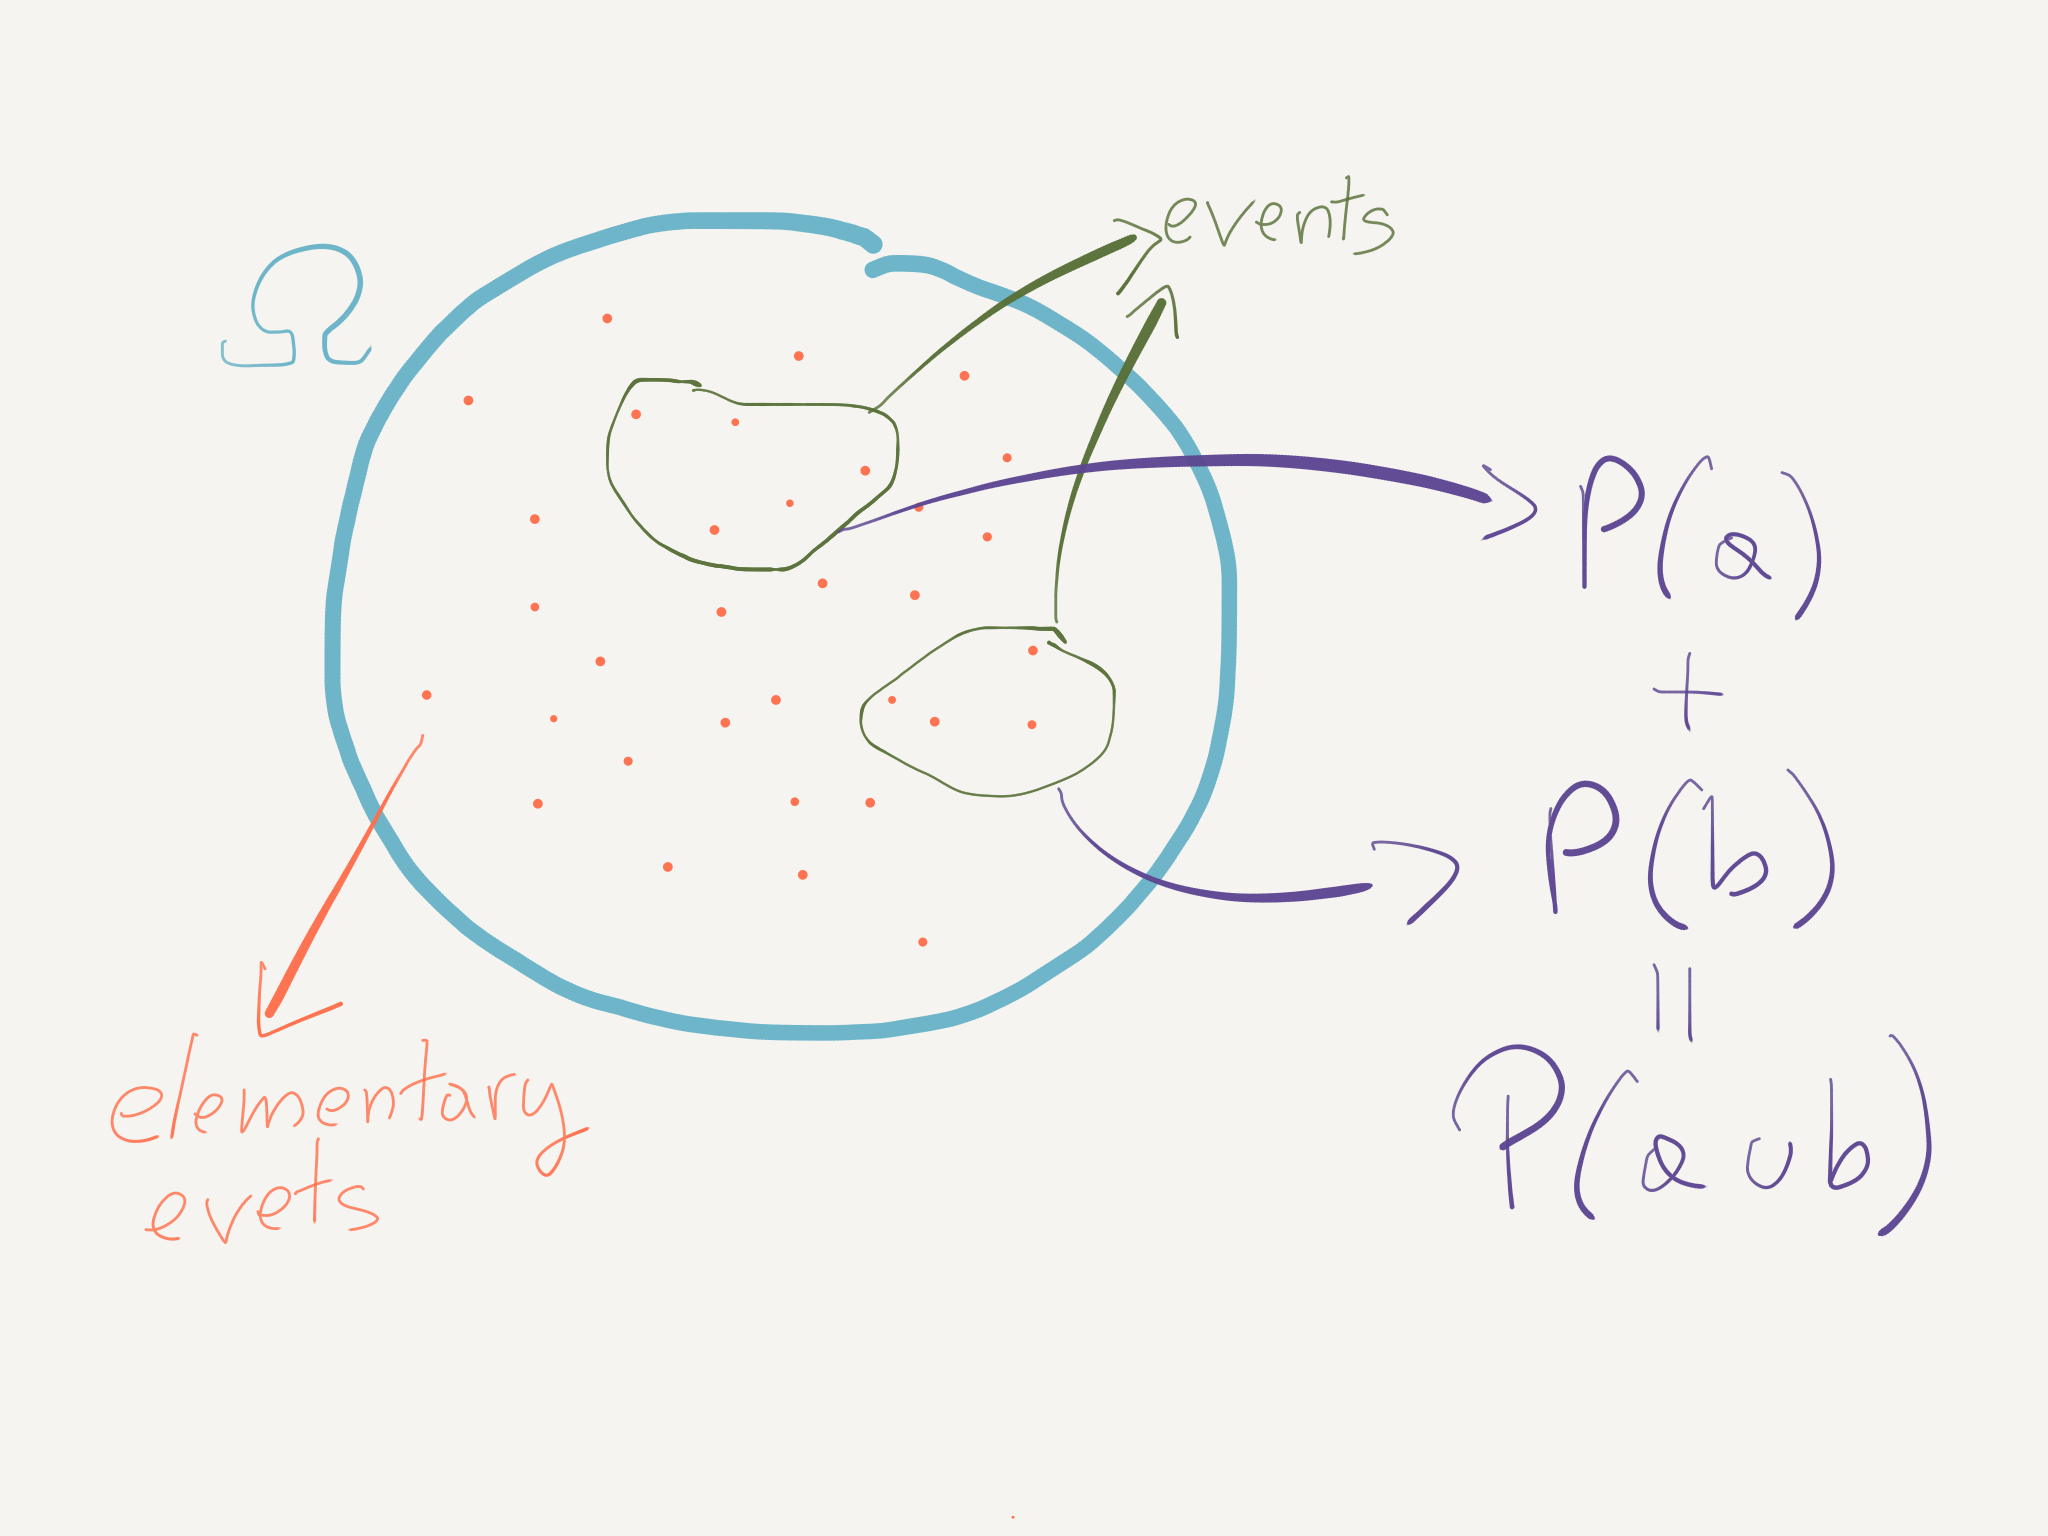
\includegraphics[width=5cm]{prob.jpg}

\end{frame}

\begin{frame}
  \frametitle{Random variables}

  \begin{block}{Random variable}\fs
    A (measurable) function $\Omega \to X$ from sample space to some set $X$.
    It maps ``random experiment outcomes'' to some mathematically tractable objects.\\
    \remark{e.g. real numbers, but can be other things too.}

    $\mathcal R(\Omega)$ -- the set of all random variables on $(\Omega,
    \mathcal{E}, P)$.
  \end{block}

  \pause

  \begin{block}{Expected value}\fs
    If $r \in \mathcal R(\Omega)$ is a random variable, then
    \begin{equation*}
      \mathbb E(r) = \int_\Omega r(x) d\alert<5->{p(x)}
                   \uncover<3->{ = \int_\Omega r(x) \alert<5->{p(x)} dx}
                   \uncover<4->{ = \sum_{x \in \Omega} r_x \alert<5->{p_x}}
    \end{equation*}
    is called \alert{expected value} of random variable $r$.
  \end{block}

  \onslide<5->{Denote by $\mathcal R^*(\Omega)$ set of all \emph{expectations}.}

\end{frame}

\begin{frame}
  \frametitle{Getting rid of sample space}
  \begin{center}
    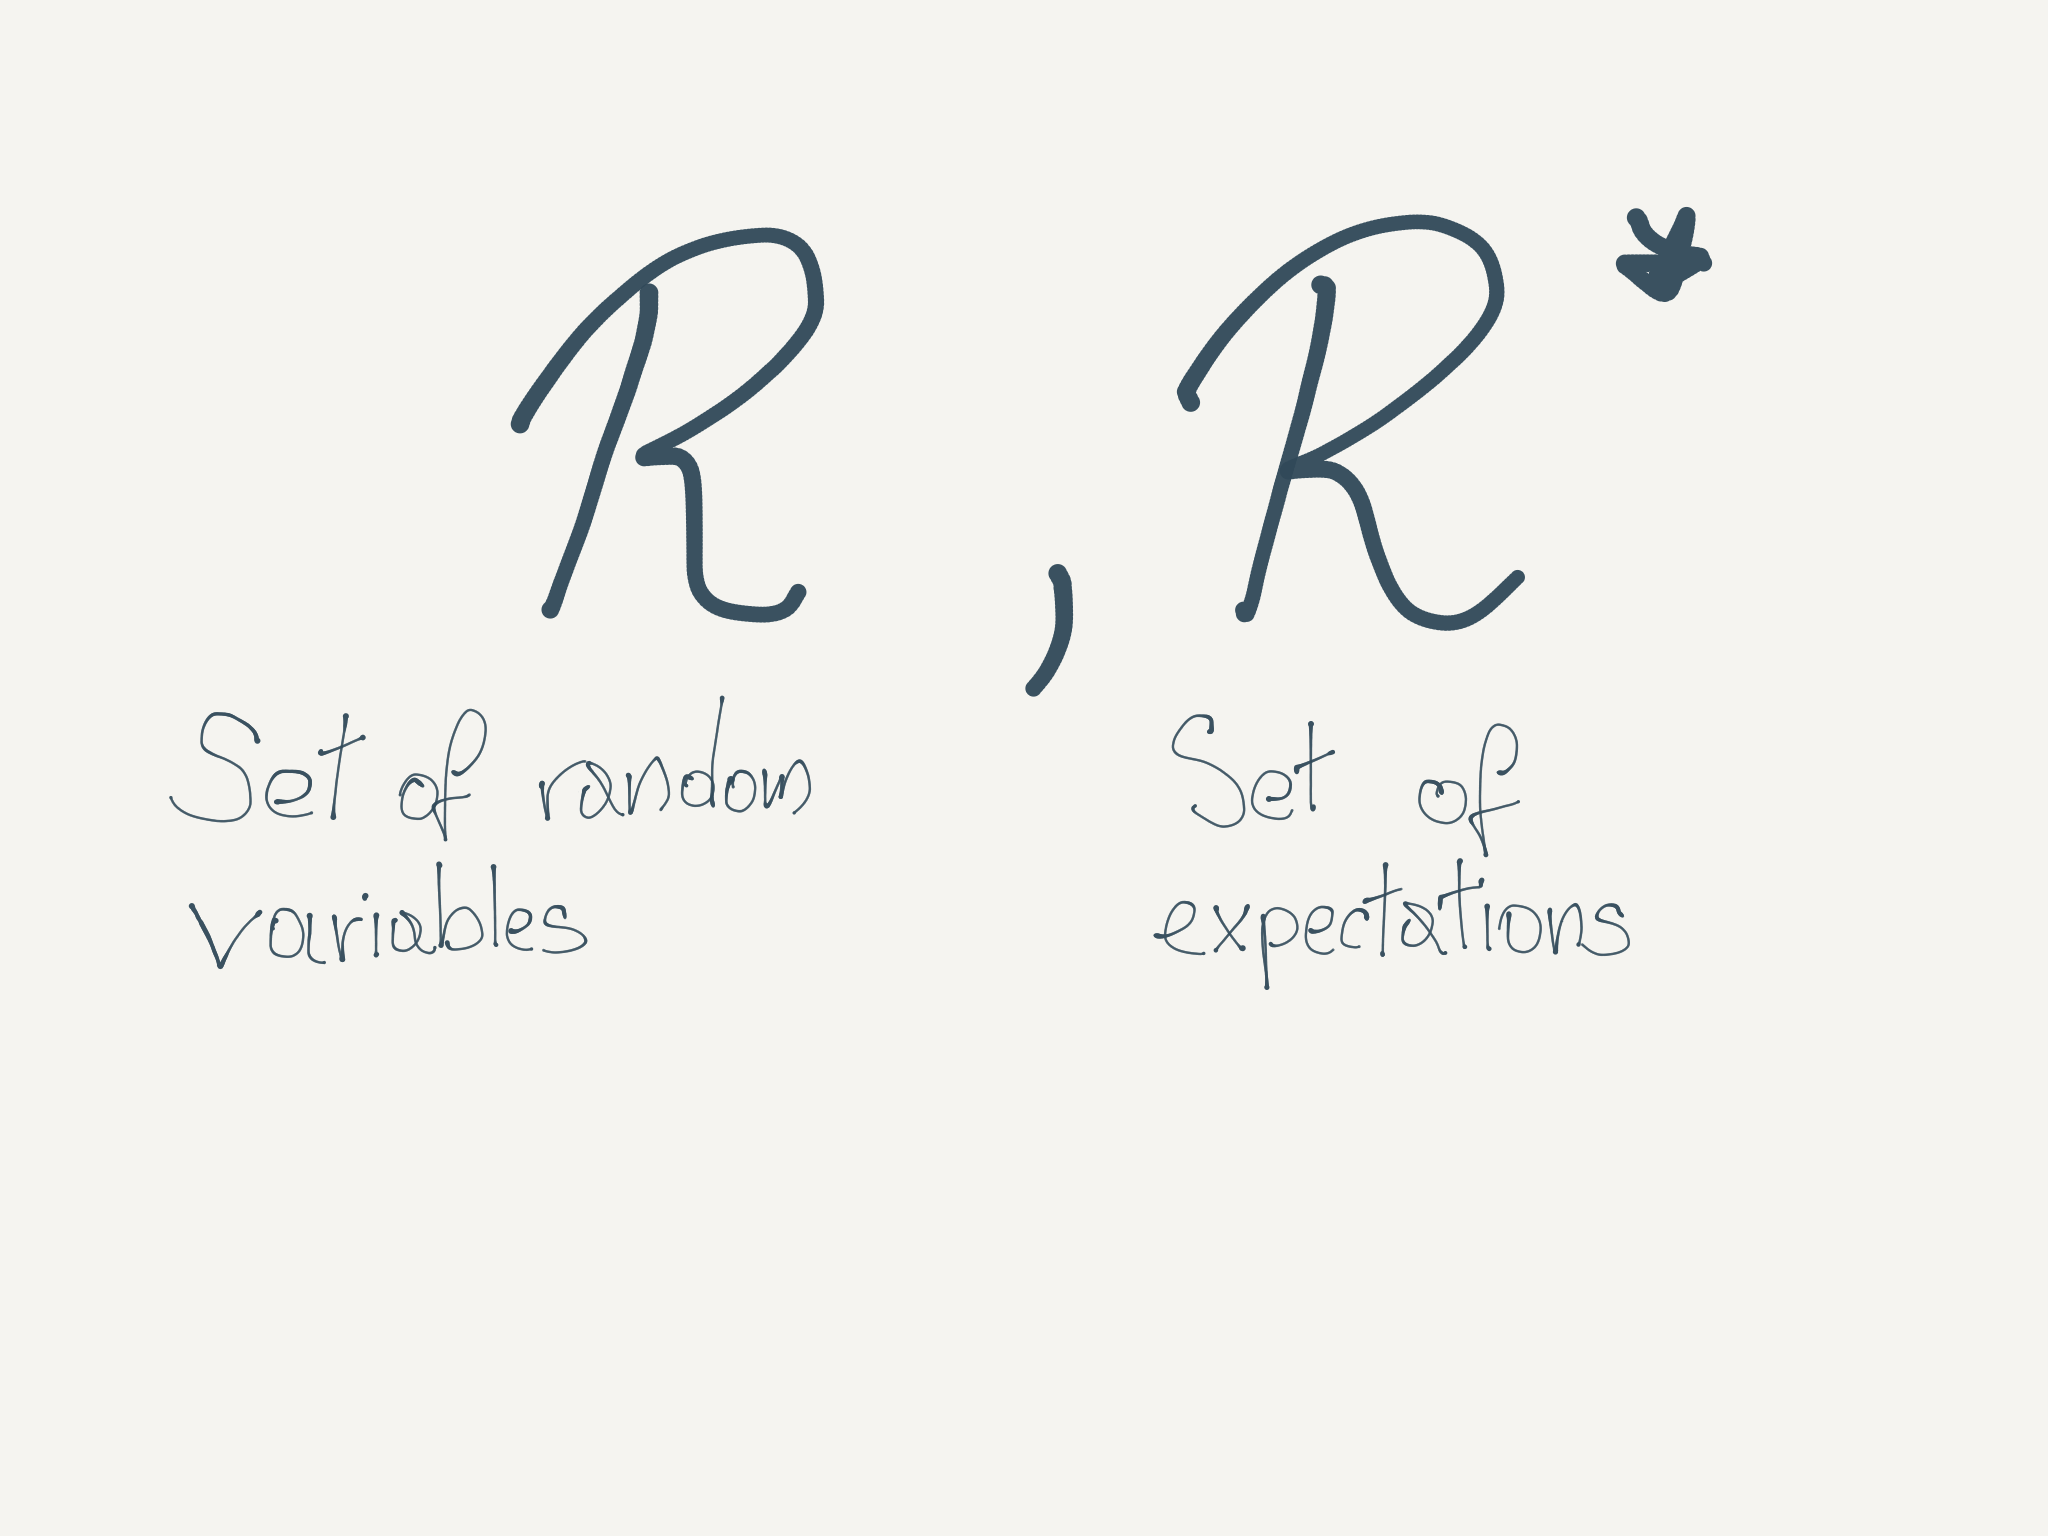
\includegraphics[width=5cm]{prob2.jpg}
  \end{center}

  $(\mathcal R, \mathcal R^*)$ the pair of (set of random variables, set of
  expectations) is totally sufficient to formulate all probability theory.

  Note that this does not mention $\Omega$!

\end{frame}

\section{Expressing idea in pseudo-Haskell}

\begin{frame}[fragile]
  \frametitle{Random variable type}

\begin{minted}{haskell}
type RVar a = Ω -> a -- random variable of type a
\end{minted}
  \pause
\begin{minted}{haskell}
instance Functor RVar where
    fmap :: (a -> b) -> RVar a -> RVar b
    fmap f rv = f . rv
\end{minted}

\pause
  Let's just substitute for \verb|RVar|:

  \mint{haskell}|fmap :: (a -> b) -> (Ω -> a) -> (Ω -> b)|

  \pause
  We can easily verify functor laws:

\begin{minted}{haskell}
fmap id rx = id . rx = rx
\end{minted}
  \pause
\begin{minted}{haskell}
fmap (g . f) rx = (g . f) . rx
(fmap g . fmap f) rx = fmap g (fmap f rx) = fmap g (f . rx) = g . (f . rx)
\end{minted}
\end{frame}

\begin{frame}[fragile]
  \frametitle{Random variable type}
  It's a monad too, in pseudo-code:

\begin{minted}{haskell}
type RVar a = Ω -> a | (Ω,Ω) -> a | (Ω,Ω,Ω) -> a | ...

instance Monad RVar where
    return :: a -> RVar a
    --        a -> (Ω -> a)
    return x = const x
\end{minted}
  \pause
\begin{minted}{haskell}
    (>>=) :: RVar a -> (a -> RVar b)   -> RVar b
    --     (Ω -> a) -> (a -> (Ω -> b)) -> ((Ω,Ω) -> b)
    rv >>= f = f . rv
    -- because Ω -> Ω -> b is isomorphic to (Ω,Ω) -> b
\end{minted}
\pause
\alert{We got rid of $\Omega$!}

\end{frame}

\section{The \texttt{random-fu} package}

\begin{frame}[fragile]
  \frametitle{Basic blocks}

  \emph{Random variable} is a basic type:
\begin{minted}{haskell}
data RVar a  -- random variable of type a

instance Monad RVar
\end{minted}

  and \emph{probability distribution} is a type-class:
\begin{minted}{haskell}
class Distribution d t where
    rvar :: d t -> RVar t
\end{minted}

  It helps to construct random variables, e.g.:
  \mint{haskell}|stdUniform :: Distribution StdUniform a => RVar a|
  \vskip-1ex
  \remark{standard uniform distribution of type \texttt{a};\\
    e.g. uniform on $[0, 1]$ interval for \texttt{Double},
    random int for \texttt{Int}, random \texttt{Bool}}
  \mint{haskell}|normal :: Distribution Normal a => a -> a -> RVar a|
  \vskip-1ex
  \remark{normal (Gaussian) random variable of type \texttt{a} with given
    mean and standard deviation;\\
    defined only for \texttt{Double} and \texttt{Float}.}
\end{frame}

\begin{frame}[fragile]
  \frametitle{Sampling random variables}

  At some point, we want to get the ``random value''.
  Random variable can be \emph{sampled:}
  \remark{types are simplified for clarity}
\begin{minted}{haskell}
  sample     :: MonadRandom  m   => RVar a -> m a
  sampleFrom :: RandomSource m s => s -> RVar a -> m a
\end{minted}

  \mintinline{haskell}{MonadRandom} is a monad that has default source of
  entropy. Instance is defined for \mintinline{haskell}{IO}.

  \mintinline{haskell}{RandomSource} is a specific source of entropy in monad
  \texttt{m}. Instances exist for standard haskell packages providing
  randomness (\texttt{mersenne-random-pure64, mwc-random, random}).
\end{frame}

\begin{frame}[standout]
  A bit of live coding
\end{frame}

\section{Stochastic process}

\begin{frame}[fragile]
  \frametitle{Random walk}

  \begin{itemize}
  \item we have set of states, represented by some type, e.g.
    \mint{haskell}{type State = (Int, Int)  -- rectangular grid}
    \pause
  \item our ``system'' jumps from one state to the other, randomly:
    \mint{haskell}{jump :: State -> RVar State}
    Next state depend on current state.
    \pause
  \item we iterate process $k$-times starting from some point \mintinline{haskell}|s0|:
\begin{minted}{haskell}
run :: Int -> (State -> RVar State) -> State -> RVar State
run n t s0 = t s0 >>= process (n-1) t
\end{minted}
  \end{itemize}

  Let's put it together.
\end{frame}

\begin{frame}
  \frametitle{Snakes \& Ladders}
  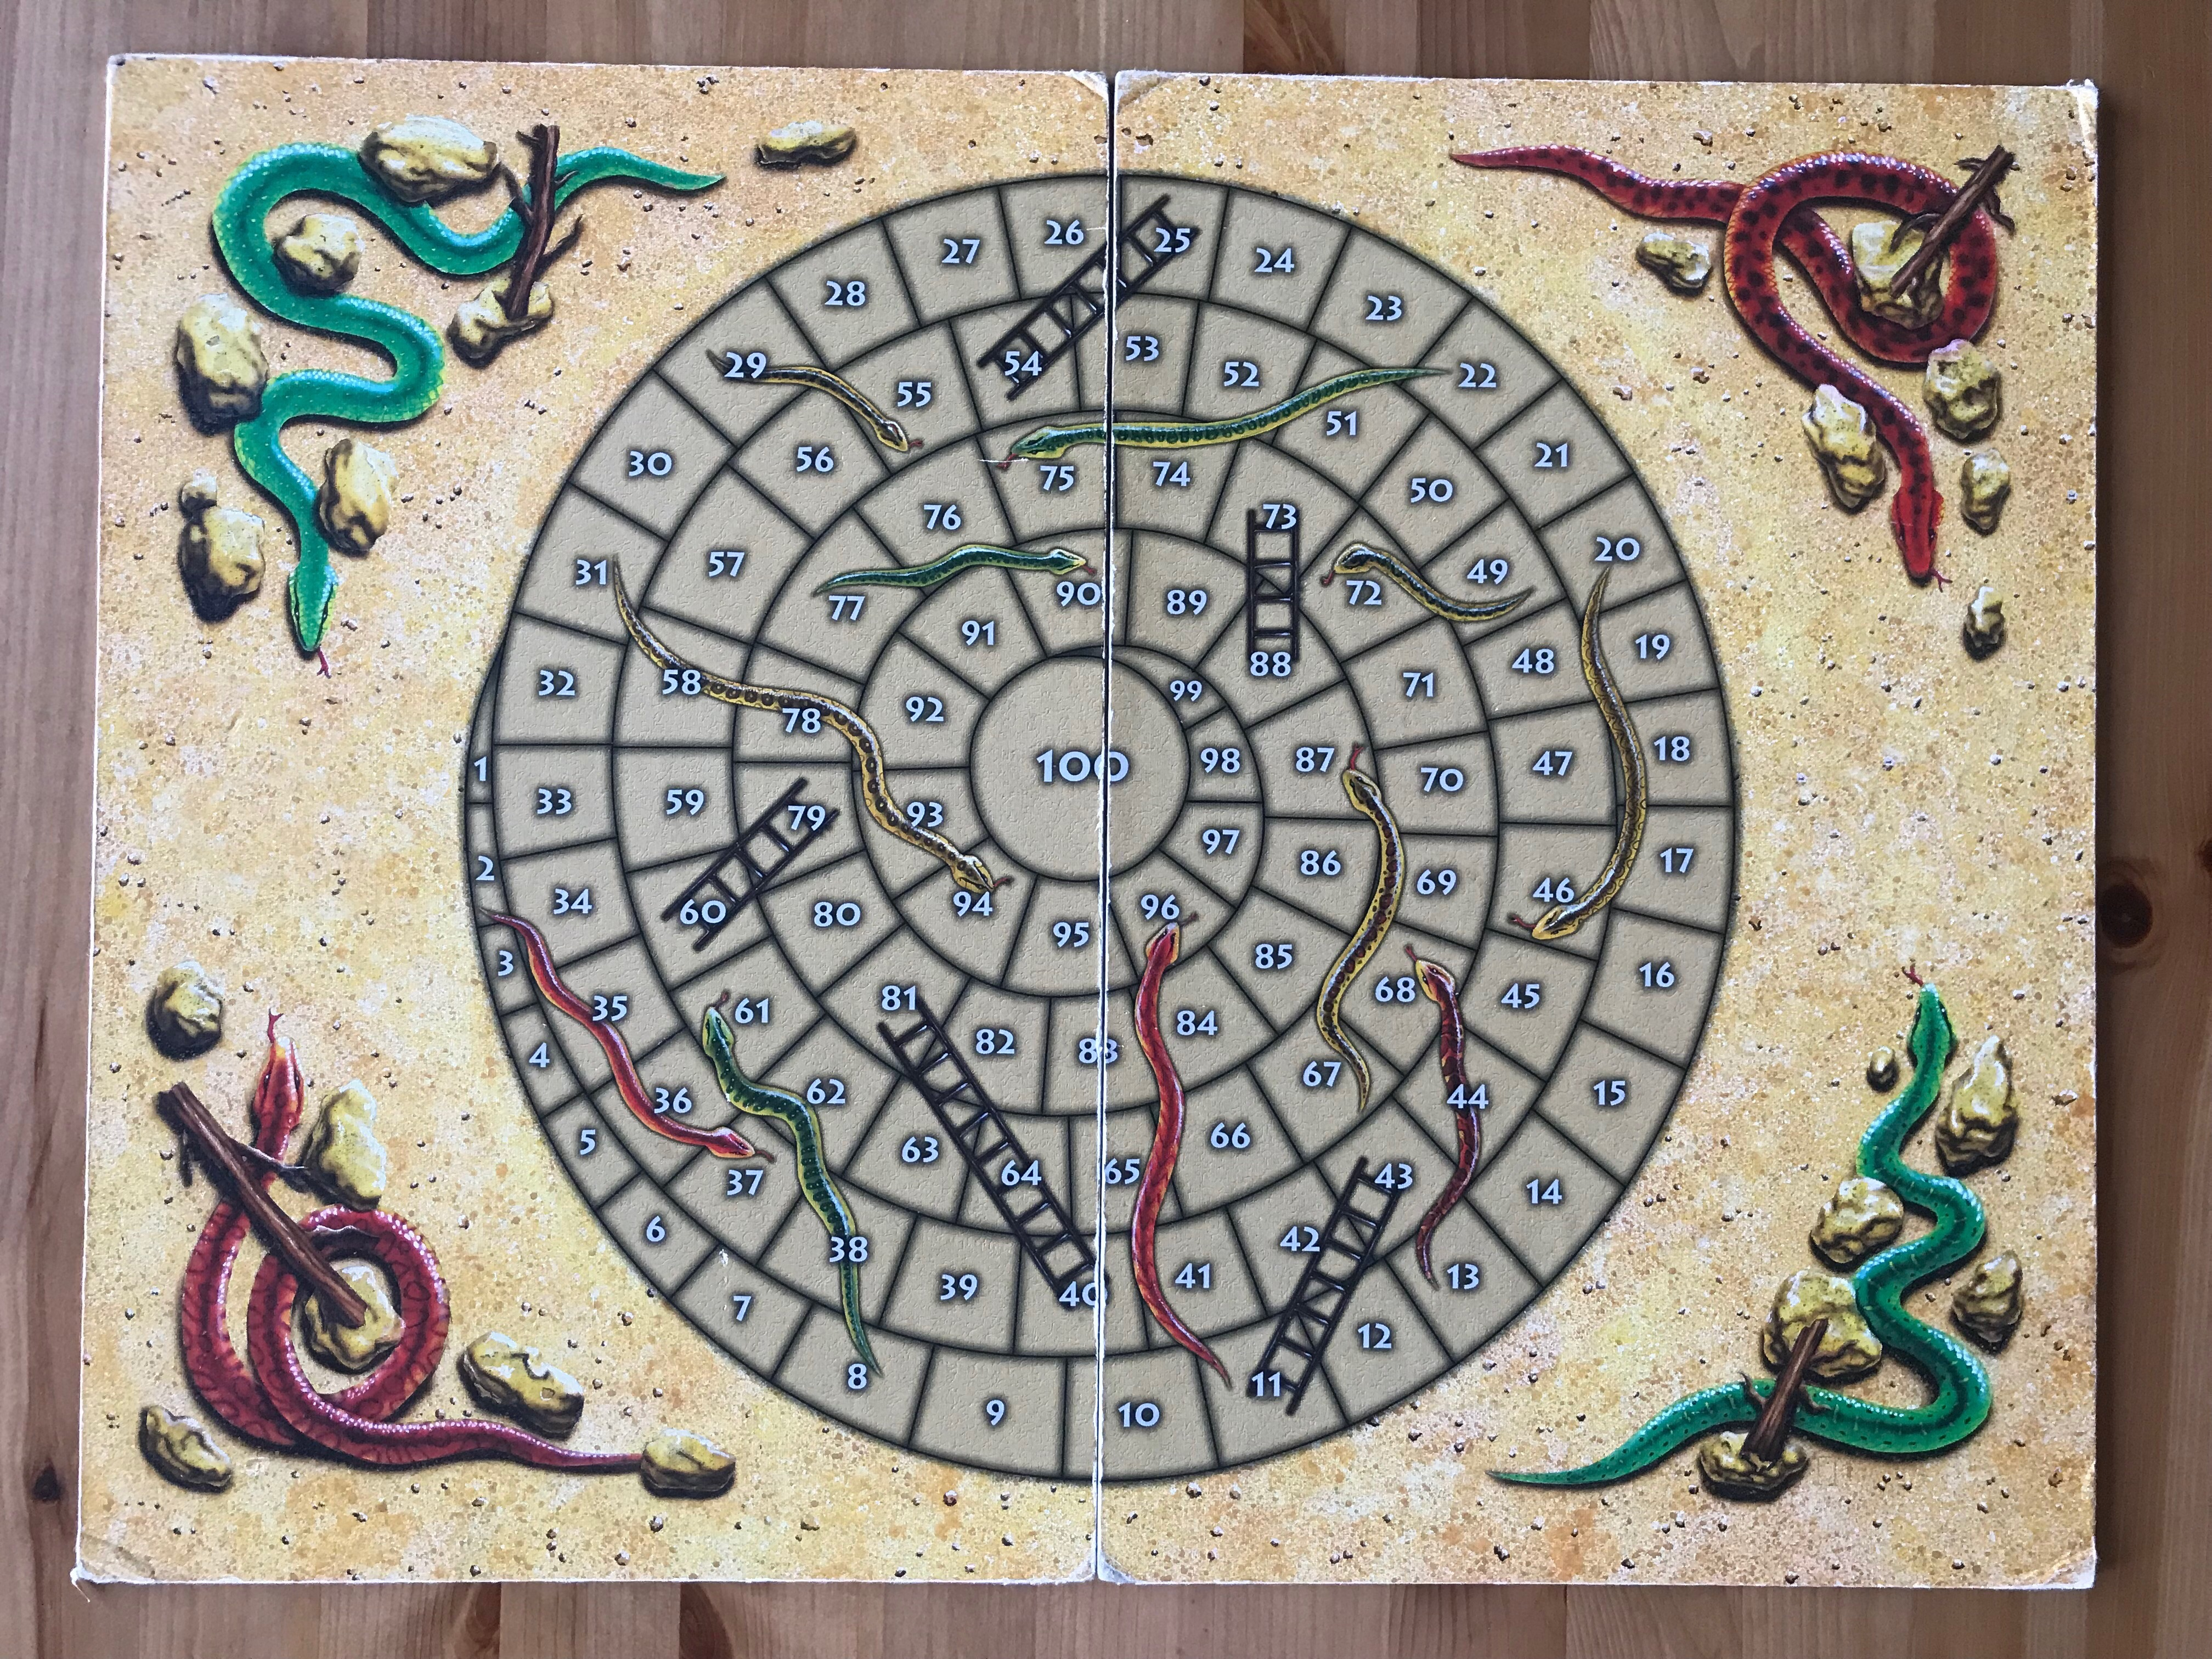
\includegraphics[width=10cm]{snakes_ladders.jpg}
\end{frame}

\section{Applications}

\begin{frame}[fragile]
  \frametitle{Classification rule mining}

  \begin{itemize}
  \item \mintinline{haskell}{Rule}
    is a predicate on a database \mintinline{haskell}{Database} (it selects rows)
    \pause
  \item we have function that transforms \mintinline{haskell}{Database} instance
    to rule selecting that particular instance.
\begin{minted}{haskell}
toRule :: Database -> Int -> Rule
\end{minted}
    \pause
  \item rules can be combined:
\begin{minted}{haskell}
(\/) :: Rule -> Rule -> Rule
\end{minted}
    \pause
  \item and scored:
\begin{minted}{haskell}
score :: Database -> Rule -> Database
\end{minted}
  \end{itemize}

    \pause

  \begin{block}{Algorithm}
    \fs
    We iteratively build result, starting with $r_0 = \bot$ being a null rule.
    Build a pool of rules $\mathrm{pool}$ by transforming each Database instance
    with positive target into rule.

    \begin{enumerate}
    \item take out randomly rule $q$ from the $\mathrm{pool}$
    \item combine it with previous rule $q' = q \vee r_{i-1}$
    \item if the score is smaller than given threshold then $r_i = r_{i-1}$
      otherwise $r_i = q'$
    \end{enumerate}
  \end{block}
\end{frame}

\begin{frame}[fragile]
  \frametitle{Classification rule mining -- implementation}

  \begin{block}{Algorithm}
    \fs
    We iteratively build result, starting with $r_0 = \bot$ being a null rule.
    Build a pool of rules $\mathrm{pool}$ by transforming each Database instance
    with positive target into rule.

    \begin{enumerate}
    \item take out randomly rule $q$ from the $\mathrm{pool}$
    \item combine it with previous rule $q' = q \vee r_{i-1}$
    \item if the score is smaller than given threshold then $r_i = r_{i-1}$
      otherwise $r_i = q'$
    \end{enumerate}
  \end{block}

\begin{minted}{haskell}
pickFromSet :: Set a -> RVar (a, Set a)

step :: Database -> Double -> (Rule, Set Rule) -> RVar (Rule, Set Rule)
step db thr (r, pool) = do
  (q, pool') <- pickFormSet pool
  return $ (update thr r q, pool')
\end{minted}
  \pause
\begin{minted}{haskell}
update :: Double -> Rule -> Rule -> Rule
update thr r q | score q' >= thr = q'
               | otherwise       = r
  where
    q' = r \/ q
\end{minted}
  \pause
\begin{minted}{haskell}
mine = Database -> Double -> RVar Rule
mine db thr = runUntil emptyPool (step db thr) (pool, nullRule)
  where
    pool = toSet . fmap toRule . filter positiveTarget $ db
\end{minted}
\end{frame}

\begin{frame}
  \frametitle{Comparision to older implementation (Python + C)}
  \begin{itemize}
  \item much simpler code base
    \begin{itemize}
    \item algorithm in Haskell version is well isolated in about 50 lines of code;
    \item previous implementation mix core algorithm with manipulation and has
      total 1715 lines of code.
    \end{itemize}
  \item much faster execution time (about 100$\times$ of real time speed-up)
  \item much easier development (took around 1 week)
  \end{itemize}
\end{frame}

\begin{frame}[standout]
\end{frame}

\begin{frame}[fragile]
  \frametitle{Benchmark MWC vs random-fu}
Task: compute mean value 10000 random double drawn from uniform distribution on
unit interval

\begin{verbatim}
|           | non-optimized [ms] | optimized [ms] |
|-----------|--------------------|----------------|
| random-fu |              1.800 |          0.890 |
| MWC       |              7.112 |          0.391 |
\end{verbatim}

MWC code is improves very much when optimization is
enabled. This suggest that both libs may on on-par
in less trivial programs.
\end{frame}

\end{document}
